\let\negmedspace\undefined
\let\negthickspace\undefined
\documentclass[journal]{IEEEtran}
\usepackage[a5paper, margin=10mm, onecolumn]{geometry}
%\usepackage{lmodern} % Ensure lmodern is loaded for pdflatex
\usepackage{tfrupee} % Include tfrupee package

\setlength{\headheight}{1cm} % Set the height of the header box
\setlength{\headsep}{0mm}     % Set the distance between the header box and the top of the text

\usepackage{gvv-book}
\usepackage{gvv}
\usepackage{cite}
\usepackage{amsmath,amssymb,amsfonts,amsthm}
\usepackage{algorithmic}
\usepackage{graphicx}
\usepackage{textcomp}
\usepackage{xcolor}
\usepackage{txfonts}
\usepackage{listings}
\usepackage{enumitem}
\usepackage{mathtools}
\usepackage{gensymb}
\usepackage{comment}
\usepackage[breaklinks=true]{hyperref}
\usepackage{tkz-euclide} 
\usepackage{listings}
% \usepackage{gvv}                                        
\def\inputGnumericTable{}                                 
\usepackage[latin1]{inputenc}                                
\usepackage{color}                                            
\usepackage{array}                                            
\usepackage{longtable}                                       
\usepackage{calc}                                             
\usepackage{multirow}                                         
\usepackage{hhline}                                           
\usepackage{ifthen}                                           
\usepackage{lscape}
\begin{document}

\bibliographystyle{IEEEtran}
\vspace{3cm}

\title{4.5.14}
\author{EE25BTECH11012-BEERAM MADHURI}
% \maketitle
% \newpage
% \bigskip
{\let\newpage\relax\maketitle}

\renewcommand{\thefigure}{\theenumi}
\renewcommand{\thetable}{\theenumi}
\setlength{\intextsep}{10pt} % Space between text and floats


\numberwithin{equation}{enumi}
\numberwithin{figure}{enumi}
\renewcommand{\thetable}{\theenumi}


\textbf{Question}:\\
 Find the equation of the line through the point $(5, 2, -4)$ and which is parallel to the vector $3\hat{i} + 2\hat{j} - 8\hat{k}$.

\textbf{Solution}:\\
\begin{table}[h!]
    \centering
    \begin{tabular}{|c|c|}
\hline
\textbf{Name} & \textbf{Value} \\ \hline
$\vec{A}$ & $\myvec{2 & 1 \\0 & 3}$ \\ \hline
\end{tabular}

    \caption{4.5.14}
    \label{table 4.5.14}
\end{table}\\
\text If the direction vector of the line is $\vec{A}$ and is passing through $\vec{B}$ then, \\
Equation of the line is: $\vec{X}$ = $\vec{B}$ + $\lambda$ $\vec{A}$\\
Given,
\begin{align}
\text{The line is parallel to the vector}
\begin{pmatrix}3 \\2 \\-8\end{pmatrix}
\end{align}
\begin{align}
\therefore \text{Direction vector is: } \lambda\begin{pmatrix}
3 \\
2 \\
-8
\end{pmatrix}
\end{align}

Equation of the line :-
\begin{align}
\vec{x} = \begin{pmatrix}5 \\2 \\-4\end{pmatrix} + \lambda \begin{pmatrix}3 \\2 \\-8\end{pmatrix}
\end{align}
\text{Where,}
\begin{align}
\vec{x}= \begin{pmatrix}\vec{x} \\\vec{y} \\\vec{z}\end{pmatrix}
\end{align}
Hence, Equation of the line passing through $\begin{pmatrix}5 \\2 \\-4\end{pmatrix}$ and Parallel to $\begin{pmatrix}3 \\2 \\-8\end{pmatrix}$ is:\\
\begin{align*}
\vec{x} = \begin{pmatrix}5 \\2 \\-4\end{pmatrix} + \lambda \begin{pmatrix}3 \\2 \\-8\end{pmatrix}
\end{align*}

\begin{figure}[H]
    \centering
    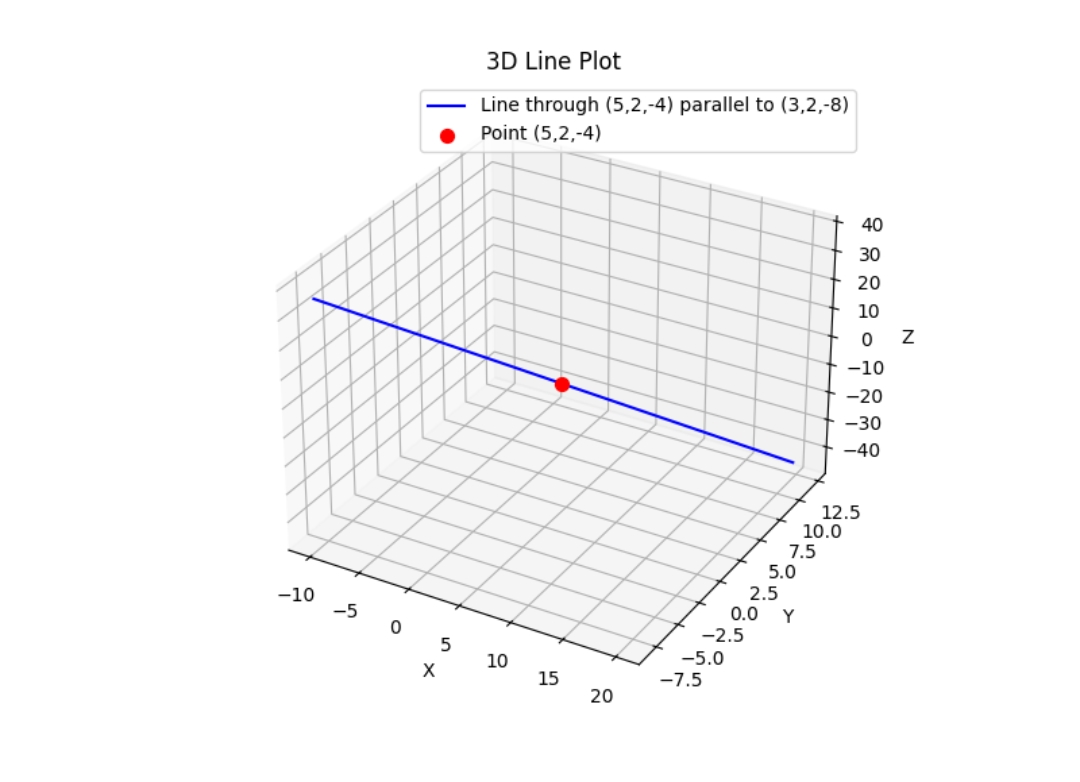
\includegraphics[width=0.8\columnwidth]{figs/line.jpg}
    \caption{}
    \label{fig:LINE}
\end{figure}
\end{document}
